

\section{State of the Art and Principles of Embryo Development Models  }

  In Chapter 1, we offered a summarized historical timeline of experiments and observations in developmental biology. Although the cited works made theoretical assumptions and proposed hypotheses about the mechanisms of development (Waddington, Needham and others had founded the "Theoretical Biology Club" in 1930), they did not contain formalized models \textit{per se} with mathematical analysis or computational simulation. No symbolic or numerical calculation was performed. In the meantime and especially recently, an increasing number of theoretical and quantitative models of development have been proposed. We review here a few important families of approaches to embryogenesis such as reaction-diffusion, morphogen gradients, cell shaping or segmentation. Far from being exhaustive, our review only intends to be a sampler of particularly relevant papers that illustrate typical modeling paradigms. Then, we extract common principles from these various methodologies and attempt to unify them toward an encompassing modeling framework of multicellular development---which is the goal of the MECAGEN project. 

\subsection{A Review of Theoretical Models of Development }

\subsubsection{Early Attempts}

  Nicolas Rashevsky is one of the founders of theoretical biology. His whole research effort was spent on formalizing biology using mathematics. For this new discipline, he coined the name "Mathematical Biophysics" in 1938 \cite{Rashevsky:1938tf}. He was the first to attempt a quantitative description of biological phenomena, and insisted on bringing theoreticians and experimentalists together to maintain close collaboration ties between them. This early interdisciplinary attitude already had its critics, as some said that he could produce "neither good mathematics nor good biology nor good physics" (from \cite{Cull:2007ib}). Concerning multicellular development, he proposed a framework to describe organisms as graphs in which vertices represented biological functions and oriented edges the interactions between them \cite{Rashevsky:1954ws}. In particular, he showed as early as 1940 that cell polarity was possible even for cell with a spherical shape \cite{Rashevsky:1940uc}. One of the earliest computer simulations of vertebrate development can be attributed to Jacobson and Gordon in 1976 \cite{Jacobson:1976cc}. They designed and calculated a mathematical model of neural plate formation. 
\begin{figure}
\begin{center}
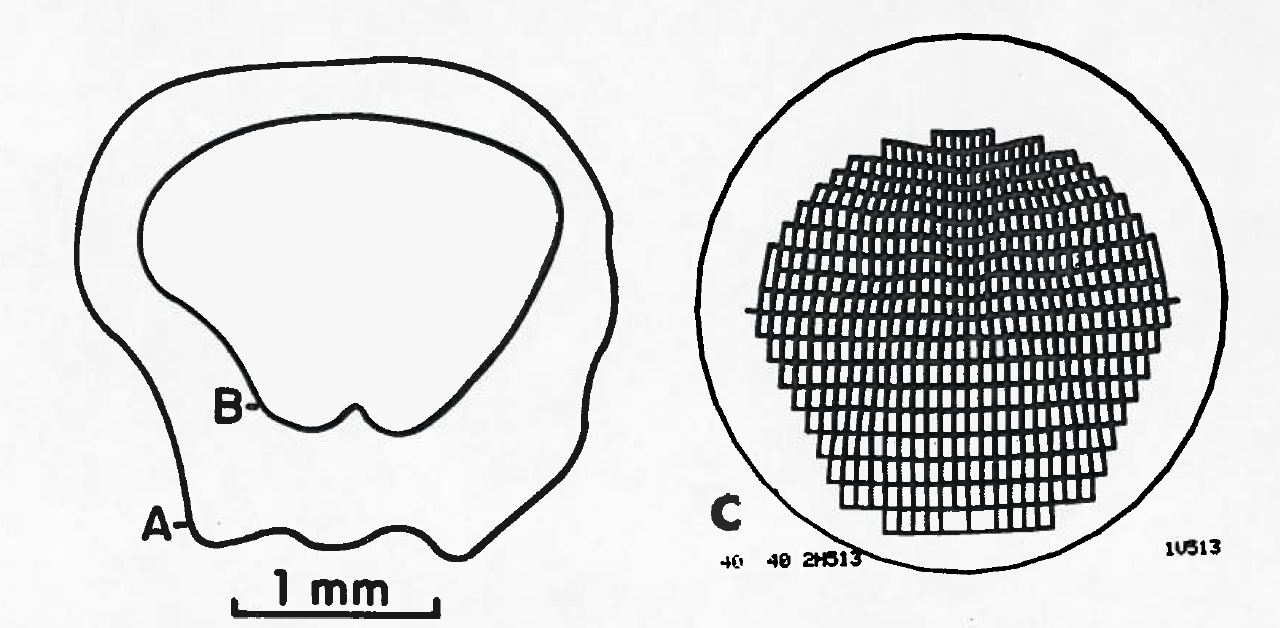
\includegraphics[width=0.5\textwidth]{../../images/biomechanics_sota/jacobson1976.png}
\end{center}
\caption{\textbf{One of the earliest computer simulations of spatial transformation during vertebrate development (Jacobson and Gordon, 1976).} "A. Appearance of the neural plate immediatly after isolation without notochord at stage 13. B. Shape attained in the same explant when controls had reached mid-neurula stage 15. C. Results of a computer simulation using shrinkage alone, which would be compared to B". Images and caption from \cite{Jacobson:1976cc}.}
\label{biomechanics_sota_jacobson1976}
\end{figure}

\subsubsection{Reaction-Diffusion Systems}

  Another historical landmark in the advent of developmental models was established by Alan Turing in 1952 with his breakthrough paper on "The chemical basis of morphogenesis" \cite{Turing:1952vn}. He proved that spontaneous order, such as stripes and spots of alternating color, could arise from the amplification of unstable fluctuations in an initially homogeneous substrate. The diffusion of two chemical signals or \textit{"morphogens"} across a biological substrate, coupled with local chemical reactions is sufficient to generate complex spatial patterns. Turing predicted six stable states in his model depending on the reaction coefficients and the rates of diffusion of the morphogens. This idea was further developed and popularized by Gierer and Meinhardt in the 1970's \cite{Gierer:1972et}. They showed that by combining "a short-range positive feedback with a long-range negative feedback", they could generate all Turing patterns. Typically, a pigmented medium such as an animal coat undergoes spontaneous symmetry-breaking by diffusion of an activator substance and an inhibitor substance with two different characteristic distances \cite{Meinhardt:1974vd}. This was also demonstrated by Young in 1984 \cite{Young:1984hd} in an abstract model of vertebrate skin patterning implemented in cellular automata, in which the random initial distribution of pigmented an non-pigmented cells determined the final equilibrium pattern. An example of more biologically realistic reaction-diffusion model can be found in Amonlirdviman et al. \cite{Amonlirdviman:2005dz}, who propose that the \textit{Drosophila} epithelium is polarized with the "planar cell polarity" (PCP) pathway in a non-autonomous manner. Reviews of reaction-diffusion systems can be found in Kondo et al. \cite{Kondo:2010bx} and Murray \cite{Murray:2001uq}\cite{Murray:2003ty}. 
\begin{figure}
\begin{center}
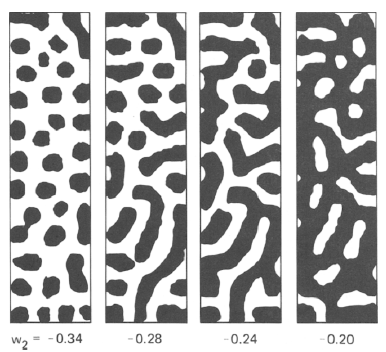
\includegraphics[width=0.6\textwidth]{../../images/biomechanics_sota/young_1984.png}
\end{center}
\caption{\textbf{Patterns produced with the activator-inhibitor model.} As inhibition is decreased (left to right), the spot pattern connects up into a pattern of stripes. Images and caption from Young, 1984 \cite{Young:1984hd}.}
\label{biomechanics_sota_young_1984}
\end{figure}

\subsubsection{Morphogen Gradients and Positional Information}

  In reaction-diffusion models, the key concept is that elements (at the molecular or cellular level) interact with their neighbors purely locally to produce ordered but repetitive patterns of contrasting activity (e.g. chemical species or pigmented cells). This family of phenomena is commonly referred to as \textit{pattern formation}. Complex patterns produced by nature have always been a source of great fascination to philosophers and scientists: ripples in sand dunes, spots in animal coats, geometric figures in plants, and a multitude of meanders, spirals, branches, and lattices observed everywhere. Most biological systems, however, distinguish themselves by strong morphological properties, i.e. an elaborate shape and body plan \textit{architecture}, which are much more sophisticated than texture-like pattern formation. Striped and spotted patterns typically result from the amplification of unstable fluctuations. Setting aside questions about the actual existence of activator and inhibitor “morphogen” agents, it remains that the pattern formation phenomena covered by such models are fundamentally random and unpredictable. Are there going to be four, five or six spots? Although the patterns are often statistically homogeneous and can be described by a characteristic scale or order parameter (diameter of the spots, width of the stripes), morphological details such as position, orientation and number are not invariants of the system.  

  Thus Turing-like reaction-diffusion principles might be able to account for some pattern formation effects in biological development, such as mammal coat (Young 1984), butterfly wing spots, angelfish stripes \cite{Young:1984hd} or seashell motifs \cite{Meinhardt:1982tv}, yet these effects seem only secondary or literally "superficial" compared to the overall form of an organism. The precisely arranged body shape of animals, made of articulated segments and subparts, is not the result of free-forming random instabilities. It is a funda-mentally "guided" morphogenesis process that plays out under deterministic control from the genome. Except for very rare cases of malformation, all members of a pentadactyl mammal species reliably develop five digits, not sometimes four or sometimes six. All healthy embryos of Drosophila exhibit exactly seven bands of differentiated gene expression along the anteroposterior axis, which then give rise to 14 segments \cite{NussleinVolhard:1980wg}. Each one of these mammal digits or insect segments is independently controlled by a specific combination of genes. At every time step in the development of an embryo, a homogeneous region of the overall embryo pattern is defined as a local group of cells that have the same gene expression profile, i.e., the same dynamic regime of RNA and protein concentrations. 

  In sum, biological forms are not statistically uniform. They are rich in morphological information and cannot be reduced to one characteristic scale like reaction-diffusion patterns. Some free pattern motifs (spots, stripes) can be embedded in a guided form (leopard, angelfish). Conversely, a guided form can be duplicated and distributed in free patterns (e.g. hundreds of copies of the same flower shape on the branches of one tree). Biological forms can thus combine a little free patterning with a lot of guided morphogenesis. The latter kind can be more effectively modeled through the paradigm of \textit{positional information} (PI) introduced by Lewis Wolpert in the 1960's \cite{Wolpert:1969wu} (later revisited and extended \cite{Wolpert:1989ut}\cite{Wolpert:1996tw}\cite{Wolpert:2011hw}) to account for heterogeneous and large-scale spatial patterns of cellular differentiation. At an abstract level, the key idea is simply that cells must establish long-range communication system that allows them to create to generate different parts of the organism in different locations. It is inevitable that some form of PI should be at work in multicellular organism development, embodied in various possible ways, either (1) through passive diffusion of morphogens spreading throughout the tissue and acting directly on distance cells and/or (2) through cell-to-cell intermediate-messenger signaling that would relay the signal \cite{Lawrence:2001bc}\cite{Lander:2002uo}\cite{Tabata:2004bp} (Fig. gradient_tabata_2004). Several experimental techniques have been developed to study the modes of propagation of the morphogens \cite{Kicheva:2012fw}. Both mechanisms give rise to concentration \textit{gradients}, either in the extra-cellular matrix (ECM) or in the cells' cytoplasm. In effect, PI is a genuine \textit{coordinate system} that self-organizes by decentralized chemical signaling among cells. Recurring at multiple levels of details in a (non-self-similar) fractal fashion, it constitutes the basis of an entire "hidden geography" for the embryo, following Enrico Coen's words \cite{Coen:1999wy}. 
\begin{figure}
\begin{center}
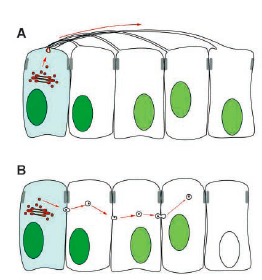
\includegraphics[width=0.4\textwidth]{../../images/Development_Review/theoretical_model/gradient/tabata_2004.png}
\end{center}
\caption{\textbf{Models for morphogen transport.} (A) A model for cytonemes. Cells at the periphery of the imaginal disc extend long processes, cytonemes, towards the AP border, where Dpp is expressed (light blue). (B) A model for argosomes. The basolateral membranes of imaginal disc cells vesiculate and travel throughout the disc epithelium. Image and caption from Tabata and Takei (2004) \cite{Tabata:2004bp}}
\label{gradient_tabata_2004}
\end{figure}

  A famous abstract illustration of gradient-based morphogenesis is the so-called "French flag problem", also coined by Wolpert \cite{Wolpert:1969wu}, in which three domains of different colors (blue, white, red) representing three modes of cell differentiation arise on top of a decreasing morphogen concentration profile. When the morphogen concentration crosses certain thresholds, cells start expressing other genes, i.e. change types. This type of "programmed patterning" has been the topic of many models, whether on a fixed lattice background or in combination with cell division and motion \cite{Miller:2003uv}\cite{Knabe:2008uk}. 

  However, a major issue with the reliance on concentration gradients for morphological patterning is obviously their \textit{robustness}\cite{Barkai:2009cs}. If they are supposed to determine, control, or even only influence the layout of the body plan and the structure of the organs and appendages, then precision should be a critical feature. Yet, this precision will not be found in the gradient diffusion or signal propagation themselves, as they are a highly noisy and approximative process. Rather, robustness is an emerging property of PI \textit{combined with} gene regulation (possibly via a correcting "attractor dynamics" \cite{Kauffman:1969ua}\cite{Reinitz:1995ws}) within the continually changing spatial environment of the growing organism \cite{RollandLagan:2012vr}. This puzzling question of the gradient-based patterns' "scaling invariance" as the tissue changes its size has triggered a number of research works \cite{BenZvi:2011ky}, in particular in the \textit{Drosophila} early striping and segmentation. Various mechanisms have been considered, whether through the ratio of two opposite morphogen gradients \cite{McHale:2006cf} (Fig. \ref{gradient_ben_zvi_2011}), the degradation of morphogens by nuclei slowing down as the embryo expands , the ubiquitous production of a size-dependent regulatory element \cite{Othmer:1980vg}, or an "expansion-repression" coupling between the morphogen and an additional molecule \cite{BenZvi:2011ky}. 
\begin{figure}
\begin{center}
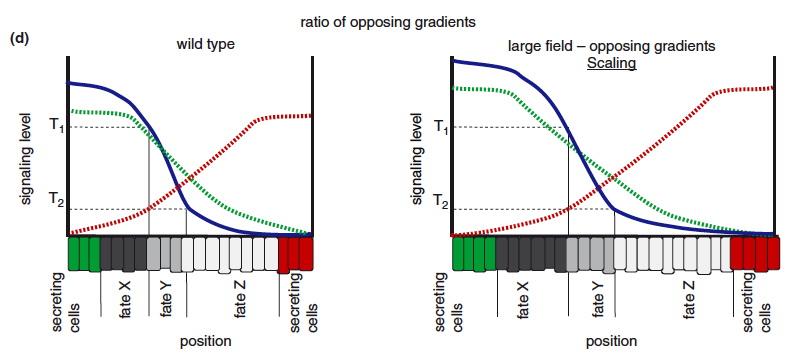
\includegraphics[width=0.4\textwidth]{../../images/Development_Review/theoretical_model/gradient/ben_zvi_2011.png}
\end{center}
\caption{\textbf{Scaling of morphogen gradients.} (d) The ratio (blue) between two gradients emanating from opposing edges of the field (green and red) can provide scaling of a signaling gradient. Left panel: wild type field; right panel: larger field. Image and caption excerpt from \cite{BenZvi:2011ky}}
\label{gradient_ben_zvi_2011}
\end{figure}

\subsubsection{Epithelial Cell Shaping and Division Patterns}

  A relatively recent interest in epithelial tissue modeling has generated a certain number of models focused on cell shaping, distribution of neighborhood sizes and division axis fields. In \cite{Gibson:2006gia}, the authors use a Markov chain model to explain the evolution of the distribution of cell shape in the \textit{Drosophila} epithelium (Fig. \ref{biomechanics_sota_epithelium}A,B). They propose that cell proliferation, and not cell packing, is responsible for the shaping of cells in monolayered epithelia. The model is generalized and compared to other organisms. Other investigators \cite{Farhadifar:2007vj} contend that physical forces, in addition to cell division, are also required to explain epithelial cell shape in the wing disc of \textit{Drosophila}. They use a vertex-based model in which vertices represent junctions between wing cells (Fig. \ref{biomechanics_sota_epithelium}C). Forces are derived from an energy function that takes into account cell elasticity, cortical tension and intercellular adhesion. The model is tested experimental data obtained by laser ablation. Patel et al. \cite{Patel:2009in} investigate two factors potentially responsible for cell proliferation: inheriting the cleavage plane orientation from mother to daughter cells, and symmetry of the division. They conclude that strong symmetry is the dominant factor explaining the distribution of shapes observed experimentally. Other vertex-based models of cell junctions can describe plant growth. For example, the particularity of the shoot apical meristem of \textit{Arabidopsis} is that it is stretched by an isotropic mechanical tension controlling the growth rate and division of the cell. A study of division patterns in this tissue \cite{Sahlin:2010eu} shows a result similar to the previous work: symmetric division is the favored factor explaining the observed cell shape distribution.  

  Sandersius et al. \cite{Sandersius:2011ug} investigate epithelium patterning before and during the primitive streak formation in the chick embryo. For them, against Gibson et al. \cite{Gibson:2006gia}, non-spatial Markov models are not sufficient to explain the histogram of number of neighbors in proliferating only epithelium. They argue that any attempt to improve biological plausibility of this type of model (e.g. with 3-sided cells or asynchronous division) induces a deviation from, instead of a refinement of, the "standard" histogram observed in various species. On the other hand, they show that their own geometrical epithelium model (based on a "Subcellular Element Model"; see Section 3.1) predicts the histogram with growth rate being the unique meaningful parameter. Escudero et al. \cite{Escudero:2011cv} introduce complex network topological measures in addition to the cells' neighborhoods and geometry. These new measures allow them to discriminate among epithelia belonging to different species, different stages of development, or genetic variants of the same species. The observed data is classified with statistical methods, allowing them to reveal the "signature" of an epithelium. The question of the interplay between cell shape and cleavage-plane orientation is reconsidered in \cite{Gibson:2011em}. 
\begin{figure}
\begin{center}
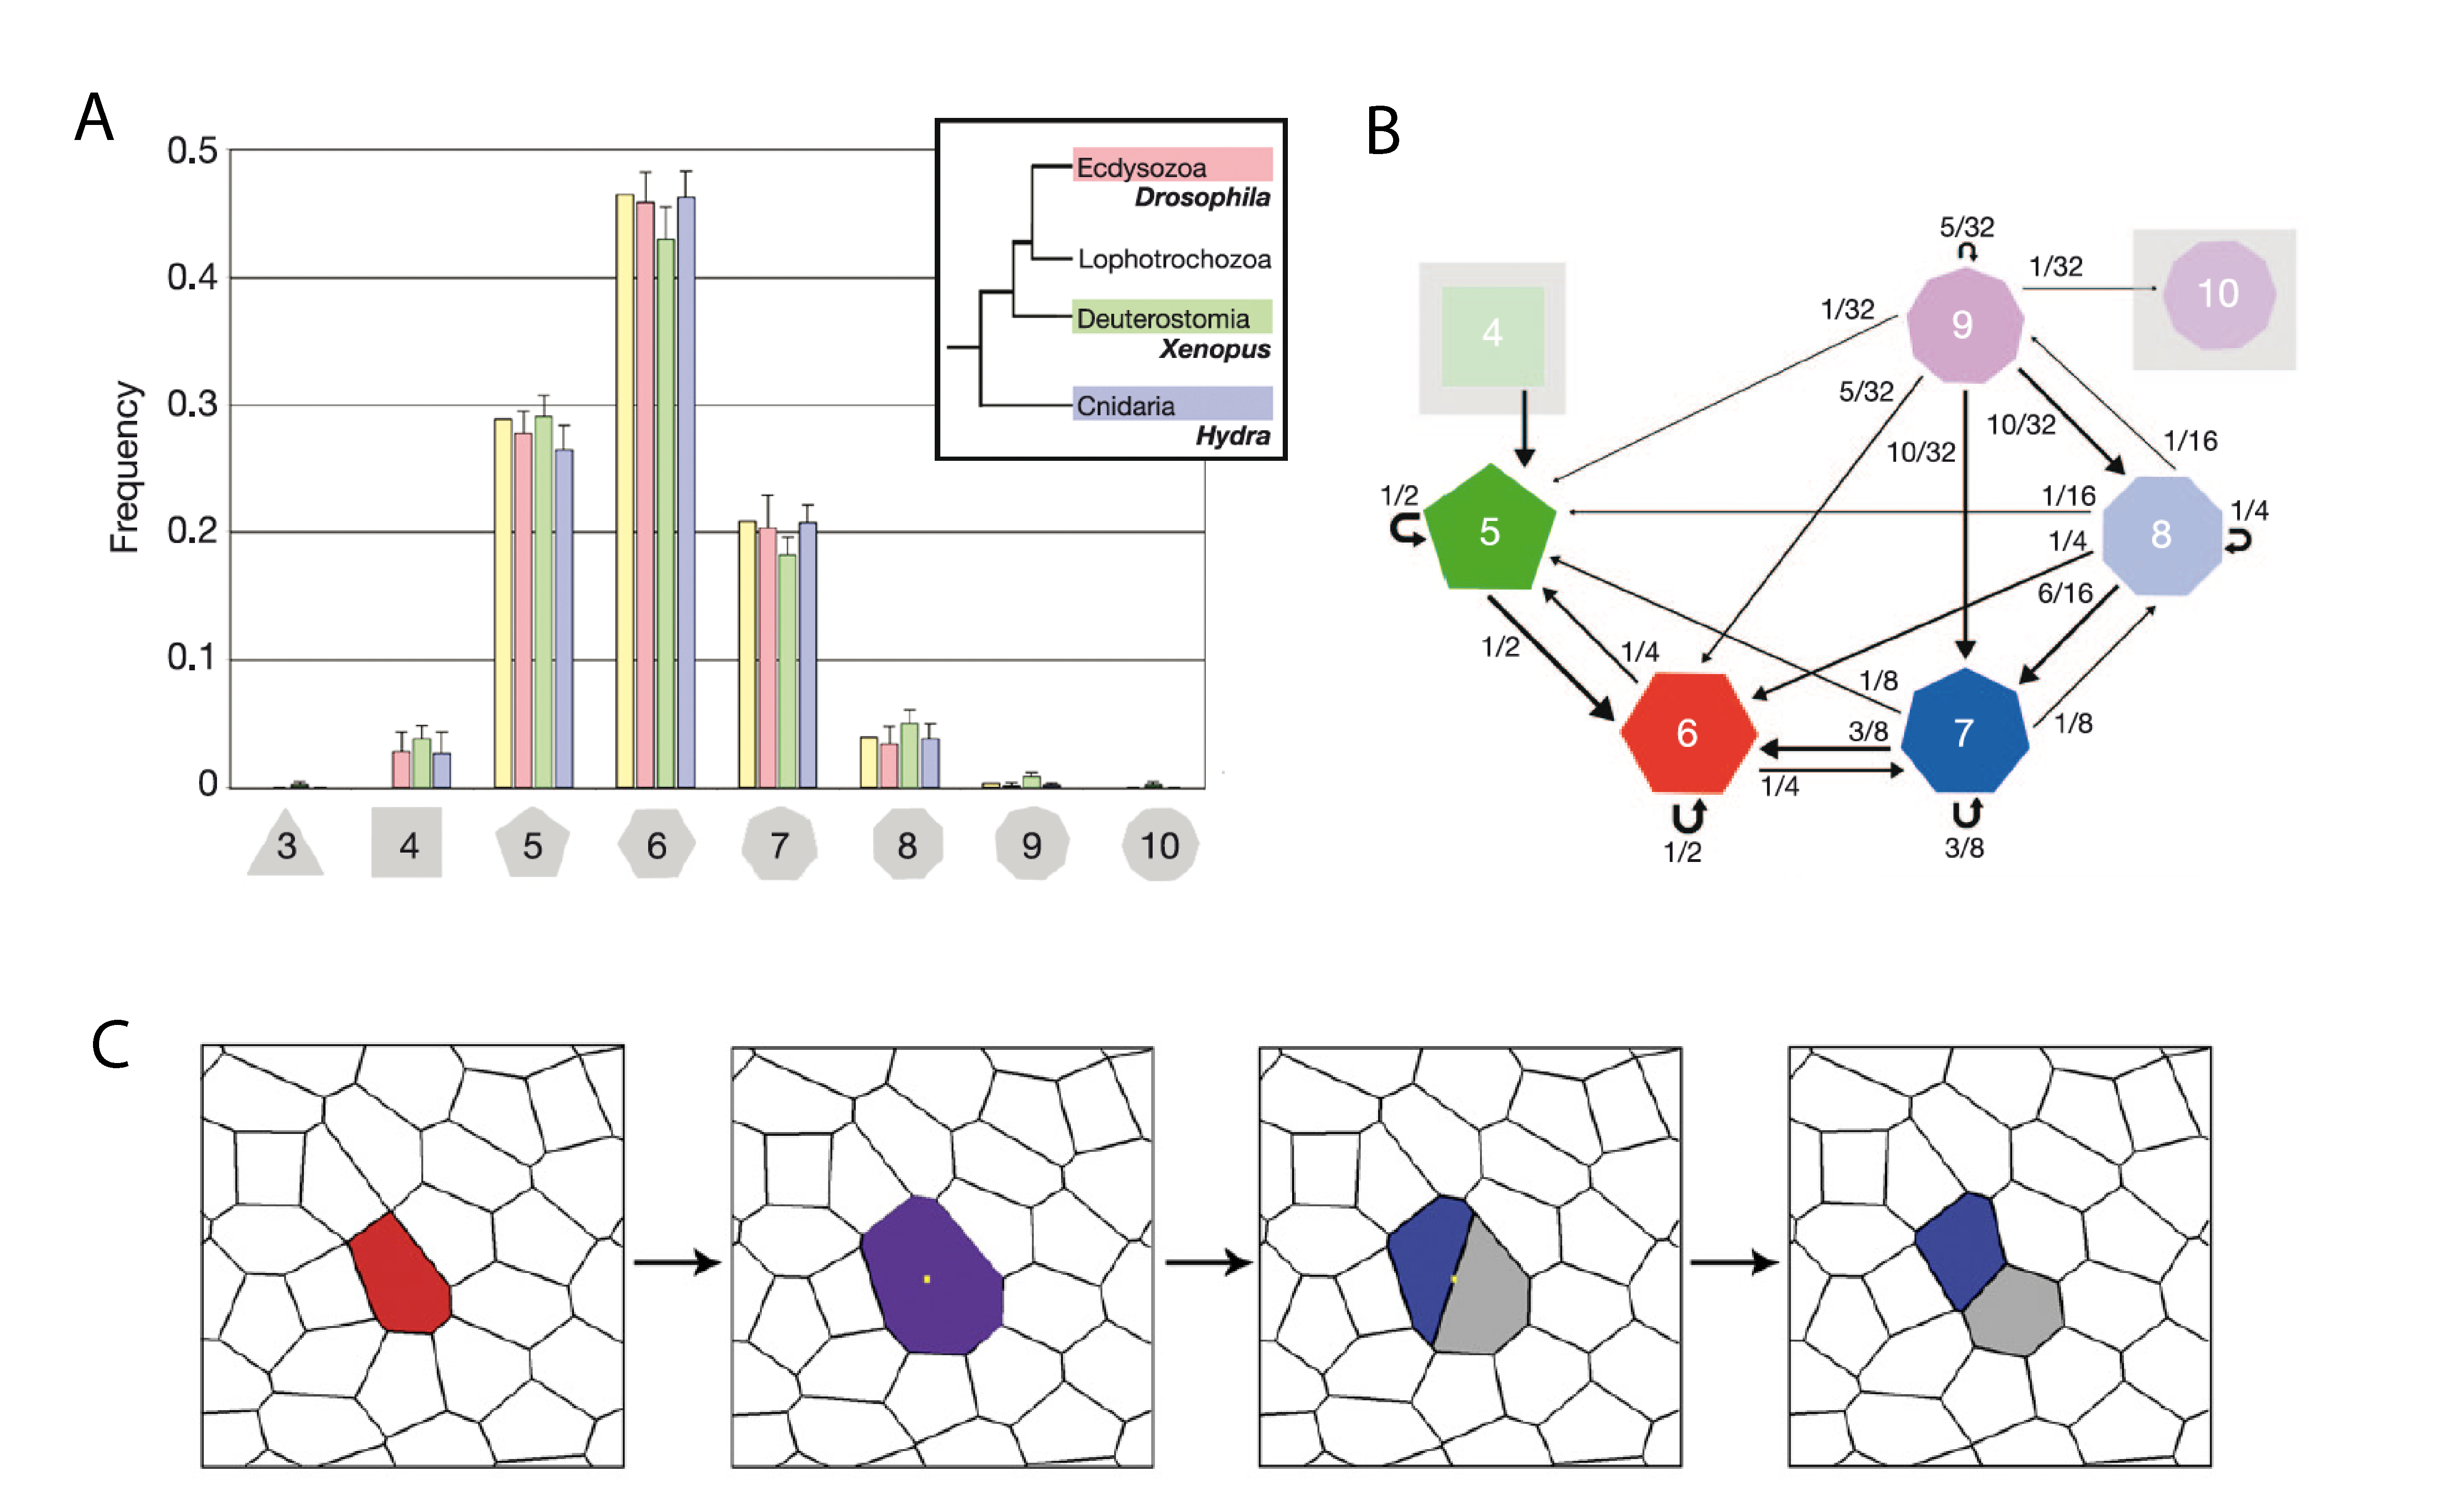
\includegraphics[width=0.9\textwidth]{../../images/biomechanics_sota/epithelium.png}
\end{center}
\caption{\textbf{Selected illustrations from the literature of epithelial cell shaping and division patterns.} A: Comparison of the distributions of polygonal epithelial cells obtained from simulation (yellow), the \textit{Drosophila} wing disc (pink), the \textit{Xenopus} tail epidermis (green) and the \textit{Hydra} epidermis (blue) \cite{Gibson:2006gia}. B: Schematized Markov chain model expressing the proliferation dynamics of polygonal cells and used in the simulation of A \cite{Gibson:2006gia}. C: Typical cell division event in a vertex-based model \cite{Farhadifar:2007vj}.}
\label{biomechanics_sota_epithelium}
\end{figure}

\subsubsection{Differential Adhesion and Cell Sorting}

  DAH, steinberg papers: 
\begin{itemize}
	\item Steinberg, M.S., 1962c. On the mechanism of tissue reconstruction by dissociated cells. I. Population kinetics, differential adhesiveness. and the absence of directed migration. Proceedings of the National Academy of Sciences of the United States of America, 48, pp.1577–1582. \cite{Steinberg:1962ww}
	\item Steinberg, M.S., 1962a. Mechanism of tissue reconstruction by dissociated cells. II. Time-course of events. Science, 137(3532), pp.762–763. \cite{Steinberg:1962tn}
	\item Steinberg, M.S., 1962b. ON THE MECHANISM OF TISSUE RECONSTRUCTION BY DISSOCIATED CELLS, III. FREE ENERGY RELATIONS AND THE REORGANIZATION OF FUSED, HETERONOMIC TISSUE FRAGMENTS. Proceedings of the National Academy of Sciences of the United States of America, 48(10), pp.1769–1776. \cite{Steinberg:1962us}
	\item Steinberg, M.S., 1963. Reconstruction of tissues by dissociated cells. Some morphogenetic tissue movements and the sorting out of embryonic cells may have a common explanation. Science, 141(3579), pp.401–408. \cite{Steinberg:1963tu}: the observation of the behavior of once dissociated and then mixed together embryonic cells resemble the one of mixed immiscible fluids. Different phase tends to cluster together to finally form two clusters, one often engulfing the other. Similarly to these fluids, Steinberg hypothesized that the cells should also minimize their surface area and this process is modulated by differences in cell-cell adhesion.   
	\item Steinberg, M.S., 1970. Does differential adhesion govern self-assembly processes in histogenesis? Equilibrium configurations and the emergence of a hierarchy among populations of embryonic cells. Journal of Experimental Zoology, 173(4), pp.395–433. 
	\item Foty, R. \& Steinberg, M., 2005. The differential adhesion hypothesis: a direct evaluation. Developmental Biology, 278(1), pp.255–263. \cite{Foty:2005wp}: the surface tension of an aggregate is proportional to the cadherin expression level.
\end{itemize}

  other papers: 
\begin{itemize}
	\item Graner, F. amp;lazier, J., 1992. Simulation of biological cell sorting using a two-dimensional extended Potts model. Physical Review Letters, 69(13), pp.2013–2016. \cite{Graner:1992ve}
	\item Glazier JA, Graner F (1993) Simulation of the differential adhesion driven rearrangement of biological cells. Phys Rev E 47: 2128–2154. \cite{Glazier:1993ck}
	\item Beysens DA, Forgacs G, Glazier JA (2000) Cell sorting is analogous to phase ordering in fluids. Proc Nat Ac Sc USA 97: 9467–9471. \cite{Beysens:2000wj}
	\item Brodland, G.W. \& Chen, H.H., 2000. The mechanics of heterotypic cell aggregates: insights from computer simulations. Journal of biomechanical engineering, 122(4), pp.402–407. \cite{Brodland:2000uu}: confront the surface tension mechanism with their finite element cell model.
	\item Landsberg, K.P. et al., 2009. Increased Cell Bond Tension Governs Cell Sorting at the Drosophila Anteroposterior Compartment Boundary. Current biology : CB, 19(22), pp.1950–1955. \cite{Landsberg:2009bp} or more recently Aliee, M. et al., 2012. Physical Mechanisms Shaping the Drosophila Dorsoventral Compartment Boundary. Current biology : CB, pp.1–10. \cite{Aliee:2012ek}
	\item Beatrici, C.P. \& Brunnet, L.G., 2011. Cell sorting based on motility differences. PHYSICAL REVIEW E, pp.1–5. \cite{Beatrici:2011vr}
	\item Zhang, Y. et al., 2011. Computer Simulations of Cell Sorting Due to Differential Adhesion. PLoS ONE, 6(10), p.e24999. \cite{Zhang:2011ca}
	\item Beatrici, C.P. \& Brunnet, L.G., 2011. Cell sorting based on motility differences. PHYSICAL REVIEW E, 84(3 Pt 1), p.031927. \cite{Beatrici:2011vr}
	\item Maître, J.-L. et al., 2012. Adhesion Functions in Cell Sorting by Mechanically Coupling the Cortices of Adhering Cells. Science. \cite{Maitre:2012cma}    Interesting, but boid based (reynolds, vicsek), no reaction from the support: Beatrici, C.P. & Brunnet, L.G., 2011. Cell sorting based on motility differences. PHYSICAL REVIEW E, 84(3 Pt 1), p.031927. \cite{Beatrici:2011vr}     reformuler le texte suivant from Mechanical control at cell–cell contacts  Cell adhesion and cortex tension are known to regulate cell–cell contact formation. Heisenberg, Paluch and colleagues now analyse the contributions of cell adhesion and cortex tension in contact formation and sorting of zebrafish progenitor cells (Science http://doi.org/jcp; 2012).  Building on previously published models of cell–cell adhesion and sorting, the authors developed a theoretical description of the shape of two progenitor cells adhering to each other. They then used dual micropipette aspiration assays to separate adhering progenitor cells from zebrafish embryos ex vivo and determined that cortex tension controls interfacial tension at the cell–cell contact, and thereby regulates cell–cell contact expansion. In contrast, cell adhesion was not involved in determining cell–cell contact size. Instead, the authors demonstrated that following mechanical separation of adhering cells, the linkage of cadherin to the actin cytoskeleton was crucial in limiting the mechanical resistance of adhesive bonds to pulling forces. The cytoskeletal anchoring of cadherins was further shown to be important for correct progenitor cell sorting within cell aggregates in vitro, and also during the segregation of progenitor cells in gastrulating zebrafish embryos in vivo. Thus, by combining theoretical, biophysical and live imaging experiments, the authors showed that cell adhesion is necessary to mechanically couple the cortices of adhering cells to support cell sorting.        
	\item cite recent papers with interfacial tension, cortical tension to modulate ...
\end{itemize}

\subsubsection{Segmentation and Somite Formation}
\begin{itemize}
	\item Intro: from Oates, A.C., Morelli, L.G. \& Ares, S., 2012. Patterning embryos with oscillations: structure, function and dynamics of the vertebrate segmentation clock. Development, 139(4), pp.625–639. \cite{Oates:2012kv}: The discovery of the segmentation clock, an oscillating genetic network in the pre-somitic mesoderm (PSM), leading the formation of somites in the elongating body axis of vertebrate embryo is the source of an active field of theoretical modeling. The phenomenon is conserved in various species and it illustrates the interplay of inner cell regulation and cell-cell communication. Cooke and Zeeman introduced a general mechanism called the \textit{clock and wavefront} mechanism which has intensively been studied since its introduction in 1976 \cite{Cooke:1976uf}. Lacking molecular grounding, it predicts the number and size of the somites from the period of the clock and the velocity of a wave travelling from the anterior to the posterior part of the axis, locking the cellular oscillators and forming a fixed periodic pattern. From then on, multiple oscillating genes, ie genes whose encoding protein and RNA follow cyclic creation and degradation, have been discovered in various species: Delta/Notch, Wnt, FGF, Hes/Her, and multiple models have been proposed to explain their interactions.
	\item    Cooke J, Zeeman EC (1976) A clock and wavefront model for control of the number of repeated structures during animal morphogenesis. J Theor Biol 58: 455–476. \cite{Cooke:1976uf}: positional information through a gradient along the AP axis is coupled with smooth cellular oscillator.  
	\item    Meinhardt, H., 1986. Models of segmentation. p.320. \cite{Bellairs:1986vo}
	\item    Baker RE, Schnell S, Maini PK (2006) A clock and wavefront mechanism for somite formation. Dev Biol 293: 116–126. \cite{Baker:2006dq}
	\item    Riedel-Kruse, I.H., Müller, C. \& Oates, A.C., 2007. Synchrony dynamics during initiation, failure, and rescue of the segmentation clock. Science, 317(5846), pp.1911–1915. \cite{RiedelKruse:2007hh}
	\item    Tiedemann HB, Schneltzer E, Zeiser S, Rubio-Aliaga I, Wurst W, et al. (2007) Cell-based simulation of dynamic expression patterns in the presomitic mesoderm. J Theor Biol 248: 120–129. \cite{Tiedemann:2007gv}
	\item    Glazier, J.A. et al., 2008. Coordinated action of N-CAM, N-cadherin, EphA4, and ephrinB2 translates genetic prepatterns into structure during somitogenesis in chick. Current topics in developmental biology, 81, pp.205–247. \cite{Glazier:2008kc}
	\item    Baker RE, Schnell S, Maini PK (2008) Mathematical models for somite formation. Multiscale Modeling of Developmental Systems 81: 183–203. \cite{Baker:2008hx}
	\item    Goldbeter A, Pourquie O (2008) Modeling the segmentation clock as a network of coupled oscillations in the Notch, Wnt and FGF signaling pathways. J Theor Biol 252: 574–585. \cite{Goldbeter:2008do}
	\item    Uriu K, Morishita Y, Iwasa Y (2010) Synchronized oscillation of the segmentation clock gene in vertebrate development. J Math Biol 61: 207–229. \cite{Uriu:2010kg}
	\item    Jensen PB, Pedersen L, Krishna S, Jensen MH (2010) A Wnt Oscillator Model for Somitogenesis. Biophys J 98: 943–950. \cite{Jensen:2010fy}
	\item    Murray, P.J., Maini, P.K. \& Baker, R.E., 2011. The clock and wavefront model revisited. Journal of Theoretical Biology, 283(1), pp.227–238. \cite{Murray:2011cy}. In addition to the posteriorly moving molecular gradient which slows the rate of the segmantation clock oscillations, the authors propose that ocillator coupling may also induce a slowing of the oscillations. Using a continuum model of oscillators, an emergent wavefront is produced with three parameters: the clock period in the PSM, the somite length, the length of the PSM. Their model predicts the distance between moving shapes of gene expression, the number of moving stripes and the oscillating period profile along the antero-posterior axis. It also states that the ratio of coupling strength explains interspecies variability and that the period profile is conserved along the antero-posterior axis.  
	\item    Hester, S.D. et al., 2011. A Multi-cell, Multi-scale Model of Vertebrate Segmentation and Somite Formation. PLoS Computational Biology, 7(10), p.e1002155. \cite{Hester:2011dc}. Builds an integrative model of the clock and wavefront mechanism. Using a wide variety of accepted "submodels" as intracellular segmentation clock, coupling through the Notch-Delta signalling pathway, FGF8 determination front, delayed differentiation or a biomechanical model of cell sorting (potts with differential cell-cell adhesion), they reveal some inconsistencies between these sub-models.   
\end{itemize}

\subsubsection{Striping in Drosophila}
\begin{itemize}
	\item wieschaus constriction apical
	\item segmentation: salazar-ciudad, kauffman, 
	\item droso : *segmentation*, genes pair-rule, gap, maternal etc. cf. Wikipedia : voir le bouquin  (mes etageres) Carroll, S. B., Grenier, J. K. and Weatherbee, S. D. 2001 From DNA to Diversity: Molecular Genetics and the Evolution of Animal Design, Blackwell Scientific, Malden, Mass
	\item von Dassow, G., Meir, E., Munro, E.M., Odell, G.M.: The segment polarity network is a robust developmental module. Nature 406, 188–192 (2000) \cite{vonDassow:2000kx}
	\item Salazar-Ciudad, I., Garcia-Fern´andez, J., Sol´e, R.: Gene networks capable of pattern formation: From induction to reactiondiffusion. Journal of Theoretical Biology 205(4), 587–603 (2000) \cite{SalazarCiudad:2000up}
	\item wing growth: - modeles *imaginal discs* et *wings* tres importants aussi : trouves en 2
	\item Cell sorting patterning in the wing : 
	\item Landsberg, K.P. et al., 2009. Increased Cell Bond Tension Governs Cell Sorting at the Drosophila Anteroposterior Compartment Boundary. Current biology : CB, 19(22), pp.1950–1955. \cite{Landsberg:2009bp} or more recently Aliee, M. et al., 2012. Physical Mechanisms Shaping the Drosophila Dorsoventral Compartment Boundary. Current biology : CB, pp.1–10. \cite{Aliee:2012ek} (already in cell sorting section)
	\item    Canela-Xandri, O. et al., 2011. Dynamics and Mechanical Stability of the Developing Dorsoventral Organizer of the Wing Imaginal Disc. PLoS Computational Biology, 7(9), p.e1002153. \cite{CanelaXandri:2011kl}
\end{itemize}

\textbf{General Review to cite in the end of the section (XXXXXX)}
\begin{itemize}
	\item Oates, A.C. et al., 2009. Quantitative approaches in developmental biology. Nature Reviews Genetics, \cite{Oates:2009kg}
	\item Lewis, J., 2008. From signals to patterns: space, time, and mathematics in developmental biology. Science, 322(5900), pp.399–403. \cite{Lewis:2008kx}
	\item Tomlin, C.J. \& Axelrod, J.D., 2007. Biology by numbers: mathematical modelling in developmental biology. Nature Reviews Genetics, 8(5), pp.331–340. \cite{Tomlin:2007gq}
	\item Reeves, G.T. et al., 2006. Quantitative Models of Developmental Pattern Formation. Developmental cell, 11(3), pp.289–300. \cite{Reeves:2006bm}
	\item Morelli, L.G. et al., 2012. Computational approaches to developmental patterning. Science, 336(6078), pp.187–191. \cite{Morelli:2012ht}
\end{itemize}

\subsection{Common Modeling Principles: Toward an Integrated Theory of Development }

  Most of the models reviewed in the previous section are focused on specific aspects of development, whether certain episodes of embryogenesis localized in space and time, or particular mechanical or genetic components of the dynamics. The ambition of the MECAGEN project, and generally the modeling community, is to integrate all these dimensions into one comprehensive, or \textit{"in toto"}, model. The benefits of stitching together various approaches and components are to push them toward a mutual adaptation and cross-validation in the perspective of building a global homogeneous and consistent framework. Typically, studies of local phenomena follow a "figure/background" template in which the object of interest is the figure and is modeled in detail, while the environment is a background and is only a rough approximation. In an integrated model, both are "figures" and are represented by rules and laws.  

  The ultimate goal is to unify what Darwin called the "endless forms most beautiful" of nature, and construe them as variants around a common theme \cite{Carroll:2006ui}. The variants are the unique genetic and epigenetic information of each species; the common theme is the developmental dynamics that this information guides and "parametrizes". The Modern Synthesis of evolution and genetics postulates this reduction in principle but has never truly modeled and explained it physically. While the attention was focused on selection, it is only during the past decade that analyzing and understanding \textit{variation} (as the generation of phenotypic innovation) by comparing the developmental processes of different species, at both the embryonic and the genomic levels, became again a major concern of biology. This is the topic of \textit{evolutionary development}, a recent and rapidly expanding field of biology nicknamed "evo-devo". Researchers realized that the genotype-phenotype pairing could not forever remain an abstraction if they wanted to understand the unique power of evolution to produce countless innovative structures. To quote Kirschner and Gerhart \cite{Kirschner:2005us}: 
\begin{quotation}  When Charles Darwin proposed his theory of evolution by variation and selection, explaining selection was his great achievement. He could not explain variation. That was Darwin’s dilemma. . .  . To understand novelty in evolution, we need to understand organisms down to their individual building blocks, down to their deepest components, for these are what undergo change. (page ix) 
\end{quotation}

  Evo-devo casts a new light on the question still little addressed by today's predominant gene-centric view of biology: To what extent are organisms also the product of complex physicochemical developmental processes not necessarily or always controlled by complex underlying genetics? Before and during the advent of genetics, the study of developmental structures had been pioneered by the "structuralist" school of theoretical biology, which can be traced back to Goethe, D’Arcy Thompson, and Waddington. Later, it was most actively pursued and defended by Kauffman \cite{Kauffman:1993uj} and Goodwin \cite{Goodwin:1994tl} under the banner of "self-organization", argued to be an even greater force than natural selection in the production of viable diversity. 

  The grand challenge of creating a universal generic model of multicellular development, however, requires solving difficult problems: dealing with multiple levels of organization (metabolites, macromolecules, cells, tissues, organs), relating one level to the next by confronting the issue of "emergence", and eventually identifying custom laws at each level---as the reductionist dream of a huge atom-based simulation is not conceivable or at best completely unpractical. It involves a mix of continuous and discrete approaches, combining analytical, statistical, and agent-based computational models. Several works have ventured to propose such integrated models at various degrees of completion and with different emphasis, whether a multiscale integration of mechanical forces \cite{Blanchard:2011hk}\cite{vanLeeuwen:2009ev}, multiscale modeling of pattern formation \cite{Grima:2008ct}\cite{Little:2011cs}, or a multi-model framework for the simulation of morphogenesis such as the CompuCell platform \cite{Izaguirre:2004vr}\cite{Cickovski:2007tj}\cite{Swat:2008di}. 

\subsubsection{Dealing with Multiple Levels of Organization }

  Although "materialism" and "physicalism" have different historical roots, their meaning today is basically equivalent. They state that everything in the natural world is physical and conforms to the action of physical matter. Moreover, the study of biological development is well within the framework of classical physics and is not concerned with more speculative domains at extreme scales such as quantum physics (dealing with objects smaller than atoms), general relativity (dealing with objects near the speed of light), or consciousness (dealing with the phenomenology of the subject). Modern science's understanding of the material world is traditionally categorized into a hierarchy of levels (Fig. \ref{leveloforganization_circle}). At the smallest scales reside subatomic particles and possibly superstrings, which create the \textit{atoms}. The atoms arrange themselves into \textit{molecules}, which represent the lowest relevant level for the study of biological development. Small molecules in turn interact to form macromolecules (DNA, RNA, proteins) and organelles. These objects constitute the basic structural units of life, the \textit{cells}, which self-assemble into tissues, composing the organs and the \textit{organisms}. Ultimately, through their social interactions, organisms form populations, ecosystems, and finally the biosphere, which represents the whole pyramid of life on Earth.  
\begin{figure}
\begin{center}
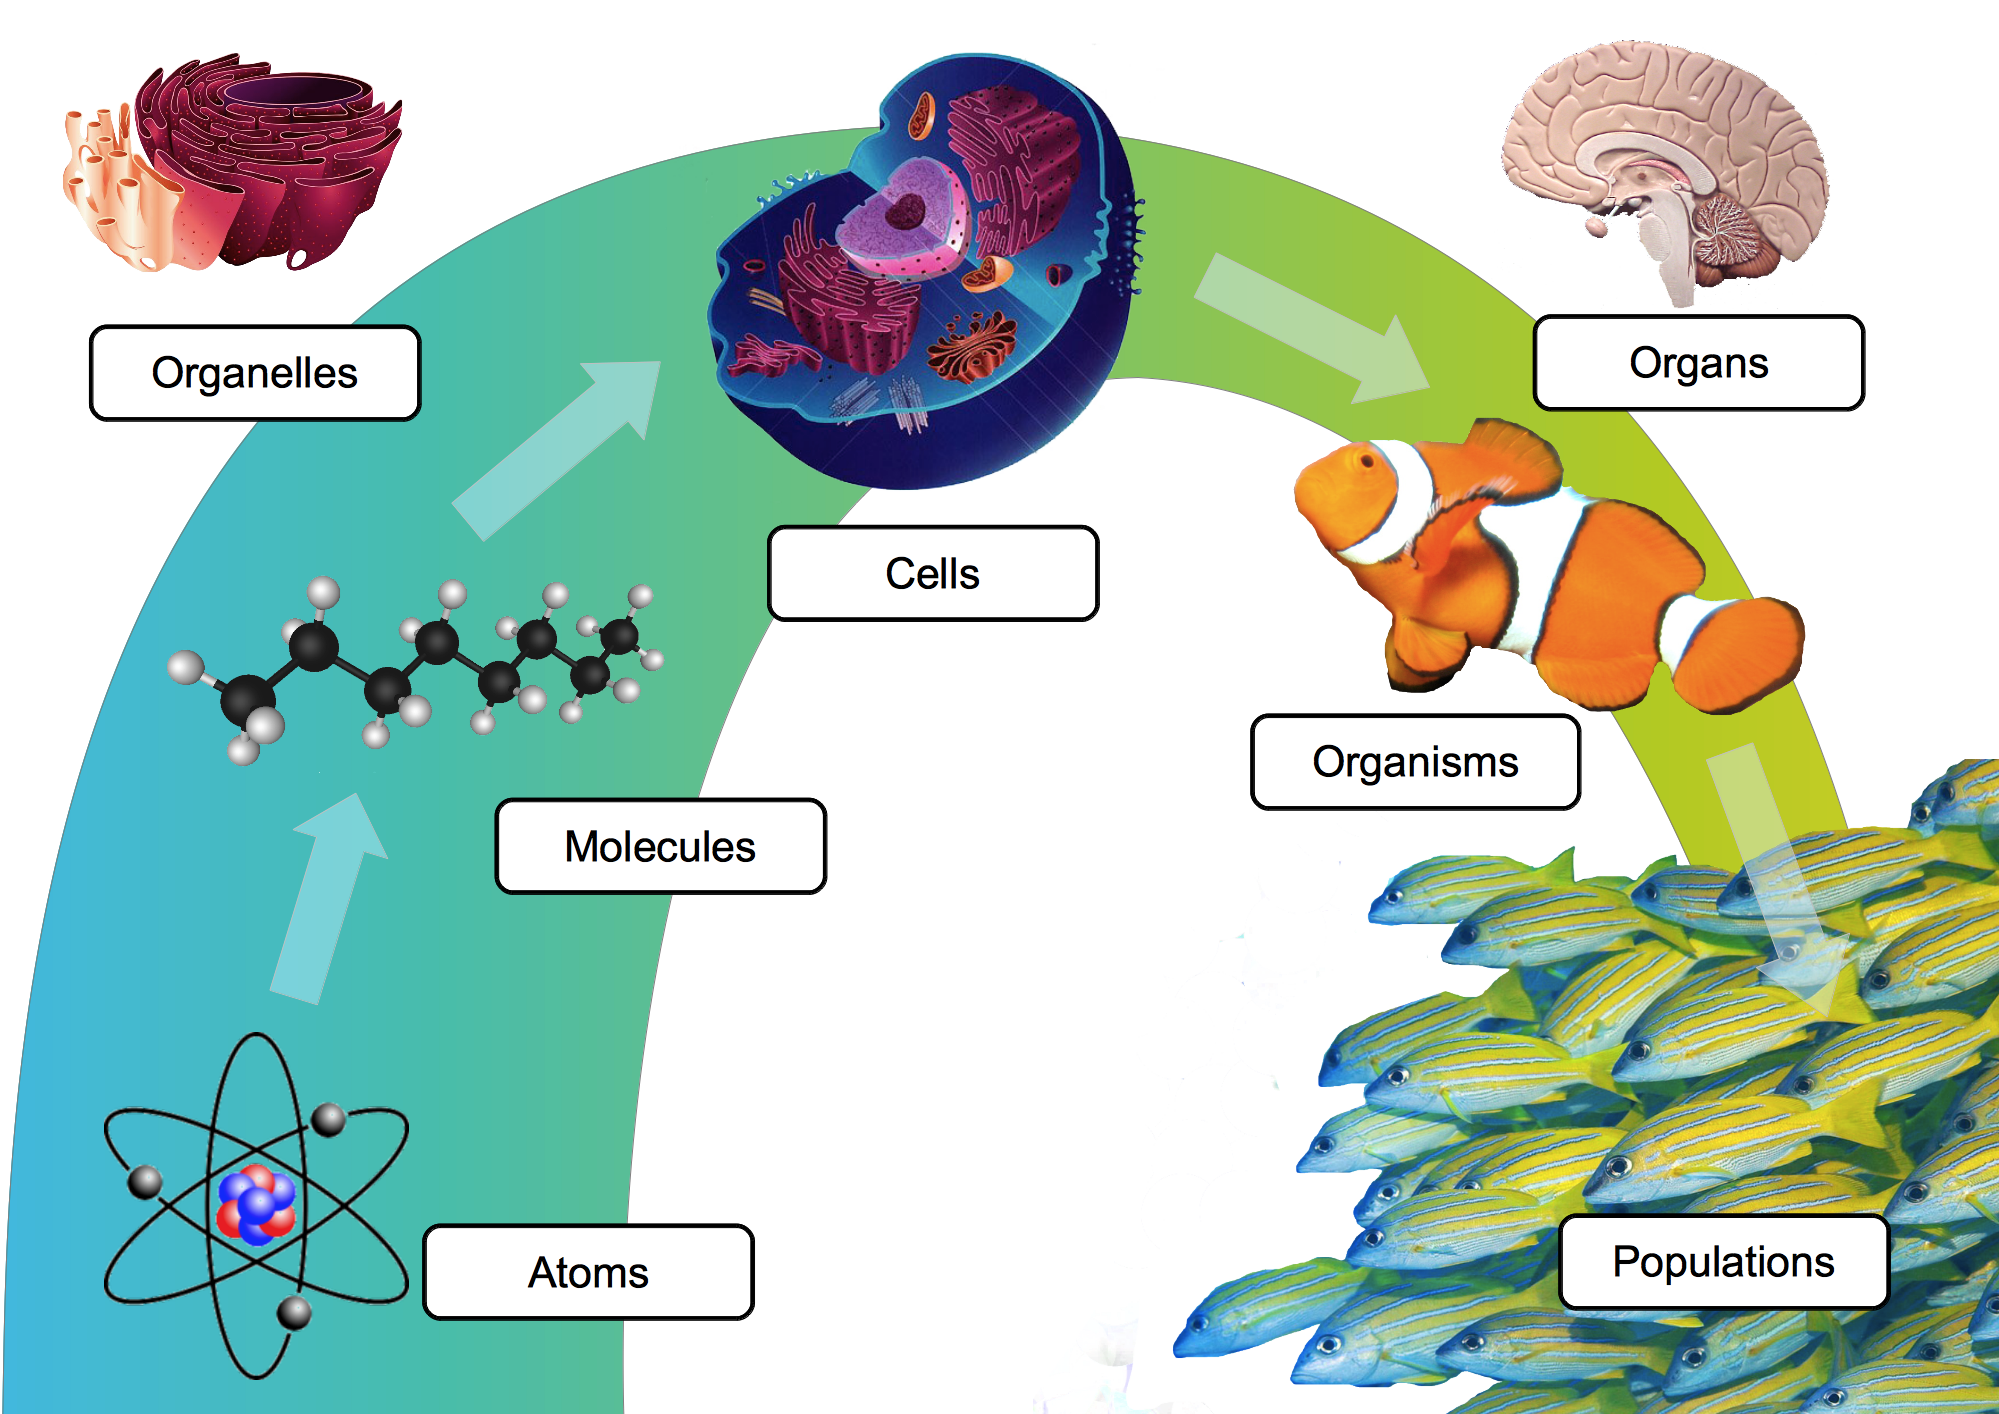
\includegraphics[width=0.9\textwidth]{../../images/levels_of_organization/leveloforganization_circle2.png}
\end{center}
\caption{Biology is studied at many levels of organization.}
\label{leveloforganization_circle}
\end{figure}

  At each level of organization, entities are \textit{complex systems} composed of a great number of small, repeated elements that interact locally and produce a collective behavior in a decentralized and self-organized fashion. They share similar structural and functional properties and are themselves internally structured as ensembles of smaller entities at a finer scale (Fig. \ref{leveloforganization_micro_macro}). For example, one cell can be modeled as a self-regulatory network of genetic switches, one social agent (insect) as a network of decision rules. Conversely, agents also interact collectively at the level of clusters or subnetworks (organs, assemblies, cliques) to combine in a modular fashion and form larger sets. Thus, from both perspectives, complex systems can often be described as “networks of networks” on several hierarchical levels. The higher levels connecting elements or clusters of elements are generally spatially extended (cell tissues, ant colonies), whereas the lower levels inside elements are generally nonspatial (gene nets, rule sets). Elements follow the dynamics dictated by their inner networks and also influence neighboring elements through the emission and reception of signals (chemical). Practically, however, complex systems models rarely involve more than two levels of organization. 
\begin{figure}
\begin{center}
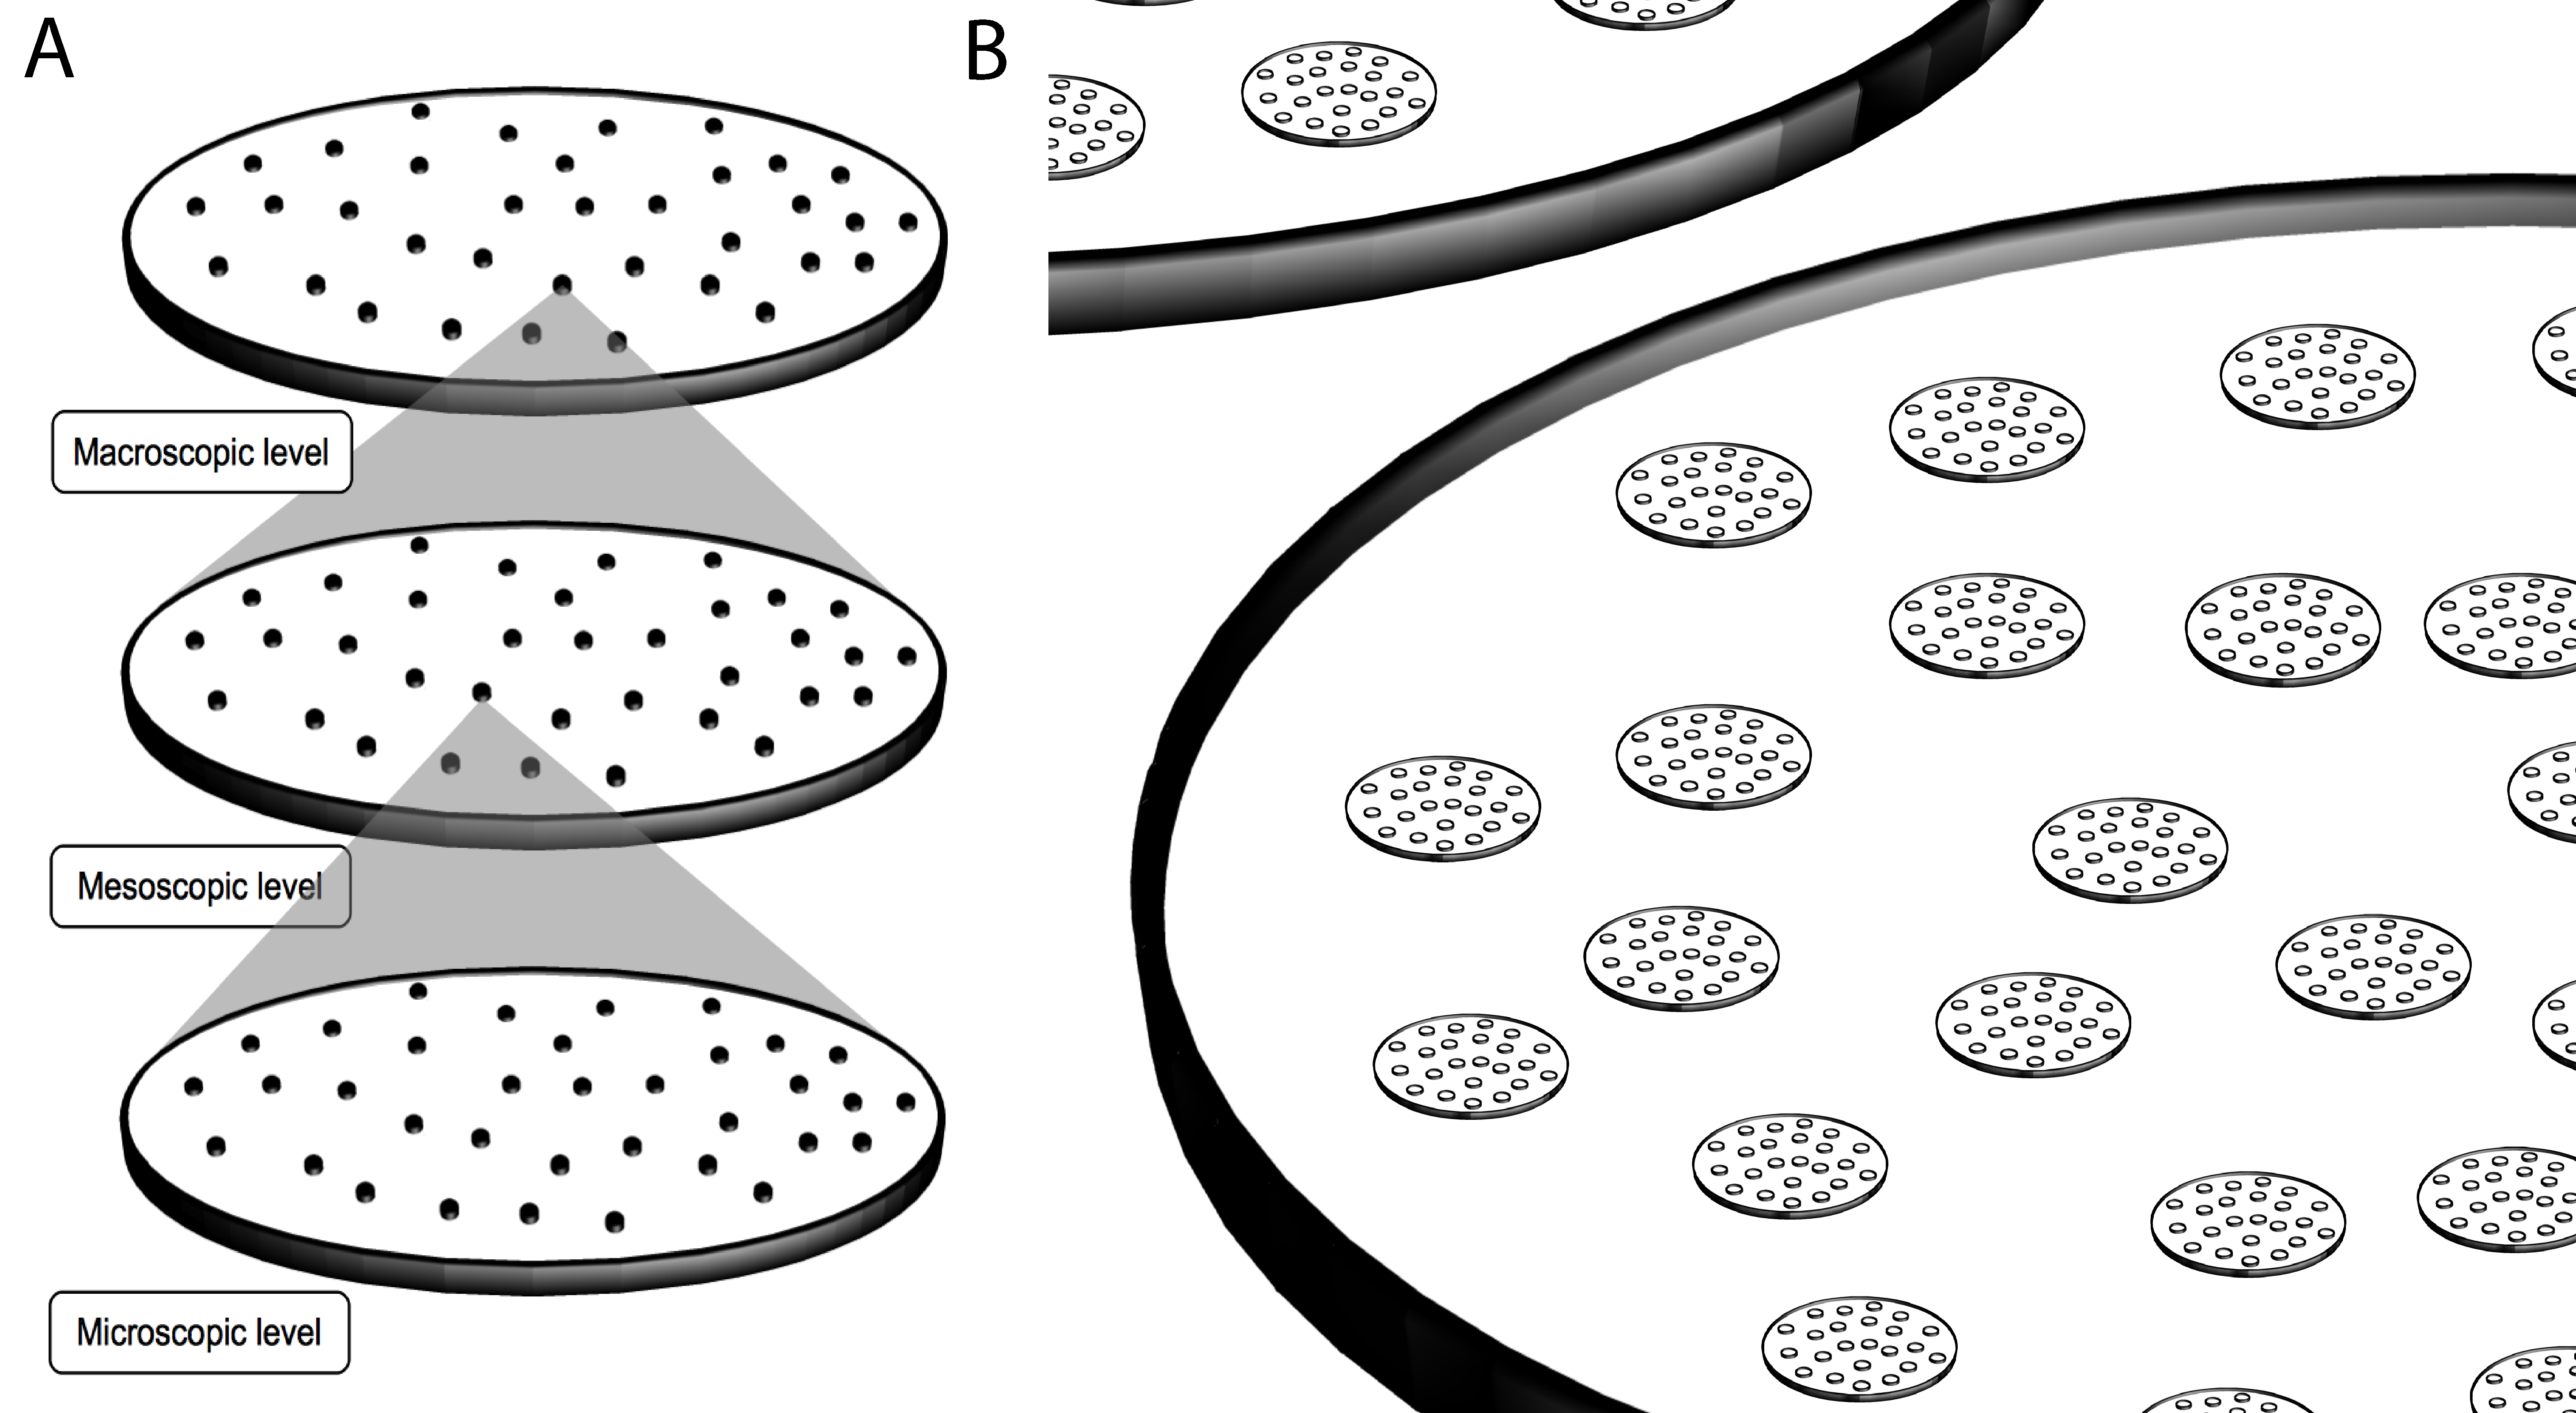
\includegraphics[width=0.8\textwidth]{../../images/levels_of_organization/micro_macro/micro_macro_julien.png}
\end{center}
\caption{\textbf{The hierarchy of level of organization of physical matter.} At each level of organization, entities are \textit{complex systems} composed of a great number of small, repeated elements. A: Level view. B: Integrated view.}
\label{leveloforganization_micro_macro}
\end{figure}

  Physicist Richard Feynman once declared that "If we were to name the most powerful assumption of all, which leads one on and on in an attempt to understand life, it is that all things are made of atoms, and that everything that living things do can be understood in terms of the jigglings and wigglings of atoms" \cite{Feynman:1964tu}. Feynman epitomizes the \textit{reductionist} school of thought according to which the behavior of any living thing can be explained exclusively in terms of its parts, subparts, and their interactions. This standpoint advocates a pure \textit{bottom-up} view of causality. On the other end of the spectrum, following the famous words of Aristotle "the whole is \textit{more} than the sum of its parts", \textit{non-reductionists} or \textit{holists} claim that understanding the world, in particular life, must rely on conceptual structures at intermediate levels adapted to the studied phenomenon. This attitude is exemplified by P.W. Anderson in this article "More is different" \cite{Anderson:1972wi}. The central concept here is that of "emergence", which as long as it has not been or cannot be reduced, justifies the very existence of all the scientific disciplines, from biology to social sciences, that are not just temporary placeholders for a yet-to-be "physics of everything", but relevant in themselves. 

  Although our personal inclination is to agree with the reductionist view, i.e. living matter could be ideally understood in terms of its atomic components, the immensity of the number of atoms exceeds the capacity of the human brain to comprehend how this type of system works. We may rely on the ever-increasing computational power of computers, yet it might only be able to "reproduce" but not "explain". Rephrasing Feynman, one could say that "everything that living things do could be 'recreated' in terms of the jigglings and wigglings of 'simulated' atoms". A whole new field of research, generally known as "computational chemistry" or "particle-based molecular dynamics", is attempting just that. Although still far from comprehensive realistic simulations, it has considerably progressed over the past few decades, boosted by the explosion of computational power. For example, Jensen et al. \cite{Jensen:2012ee} simulate the mechanisms of voltage gating in potassium channels by a molecular dynamical model whose typical simulation can process 200,000 atoms in 10 million time steps, corresponding to a total simulated time of 200 microseconds (i.e. 2 simulated femtoseconds per time step). Latest hardware technologies based on general-purpose graphics processing units (GPGPUs) can support a molecular dynamics library such as the Large-scale Atomic/Molecular Massively Parallel Simulator (LAMMPS) \cite{Plimpton:1995wl}, providing an estimated computational efficiency of 20 nanoseconds of GPU time per atom per time step (as of 2012). In this context, the above simulation of voltage gating would run about 100 hours on a single GPU, thus by extrapolation a single cell corresponding to simulated time of 10 hours would take $10^{25}$ seconds, i.e. a billion times the age of the Earth. Optimistic reductionists still rely on a continual acceleration of computing speed (possibly via novel technologies such as quantum computing) to considerably reduce this enormous duration and make it a practical tool. 

\subsubsection{Relating One Level to the Next: The Problem of Emergence}  

  The dynamics of some complex systems can be described and formalized by macroscopic equations. Typically, the goal here is to solve these equations to obtain an explicit expression of the behavior of the system over time: for example, ordinary differential equations (ODEs) of macro-variables in well-mixed systems (e.g. the law of mass action in chemical kinetics), or partial differential equations (PDEs) of local variables in spatial extended systems (e.g. the heat equation or wave equation). In certain cases, it is even possible to find the formulation of an exact solution by calculus, i.e. the symbolic manipulation of expressions (e.g. the solution of a geometric growth is an exponential function; the solution of the heat equation in homogeneous space is a Gaussian). Unfortunately, although vast, this family of analytically expressible \textit{and} solvable systems is in fact very small compared to the immense range of dynamical behaviors that natural complex systems can exhibit. Where there is no symbolic resolution of an equation, numerical analysis involving algorithms (step-by-step recipes) can be used. It involves the discretization of space into cells, and time into steps (e.g. the heat equation under irregular boundary conditions).  

  Yet, most real-world systems do not even obey clear-cut macroscopic laws. For the majority of complex dynamical systems, global ODEs and spatial PDEs are no more possible because (a) there is no law of macroscopic quantities or global metrics that can represent the behavior of the system (no "ideal gas law" $PV = nRT$ for the embryo), (b) its myriad components are irregularly placed and mobile, requiring a non-Cartesian decomposition of space (the embryo does not conform to an $x,y,z$ lattice), (c) there is a extreme degree of heterogeneity, requiring a segmentation into different classes of agents (the embryo is composed of many different cell types and behaviors), and (d) last but not least, most systems are highly adaptive, the topology and strength of the interactions depending on the short-term activity of the agents (e.g. cell migration) and the long-term fitness of the system in its environment (evolution). In short, there are no "Navier-Stokes" or "Maxwell" equations of embryogenesis. 

  A "multilevel" approach offers an alternative to the classical formalization. Instead of using a single equation ruling the behavior of a system at the macroscopic level, one can simulate the interactions of the elements at the microscopic level and observe the collective effect resulting from their aggregation. Traditionally in physics the process of deriving macroscopic laws from microscopic elementary interactions, which can be referred to as "coarse-graining" is possible with the averaging tools of \textit{statistical mechanics} (e.g. a continuum description of the clock and wavefront model of somitogenesis derived from a chain of coupled oscillators \cite{Murray:2011cy}). These approximation or "mean-field" methods use probability theory to realize the transition from the discrete paradigm of local elementary behaviors to the continuous paradigm of macroscopic descriptions. However, they are constrained by strong assumptions such as the homogeneity of the elements. For example, the collective motion of cells in a developing embryo cannot be easily assimilated to fluid mechanics.  

  Once again, a widely popular solution comes from computer science under the terminology \textit{agent-based modeling} (ABM). Historically, ABM originated from the need to model socio-economical systems too complex for analytical descriptions. Helped by the rise of computing technologies, it soon became a practical tool in many other scientific disciplines, such as ecology, biology and physics. Most of ABM is based on a combination of three types of topologies: fixed grids such as square pixels, irregular networks with long-range connections, and 2D or 3D Euclidean space supporting mobile agents and metric-based interactions. Note that the continuous/agent-based dichotomy is more conceptual than practical, as many works mix both approaches at various degrees of compromise. As A.R.A.Anderson et al. put it \cite{Anderson:2007wp}:  
\begin{quotation}  Many mathematical models of biological process that consider space explicitly, fall into one of two categories: (i) continuum population models or (ii) discrete individual based models. Discrete, stochastic interactions between individual organisms cannot be captured by the continuum approach and likewise global population interactions cannot be captured by the discrete approach. In recent years a third category of models has emerged: hybrid models which allow modellers to exploit the advantages of both continuum and discrete models.  
\end{quotation}

\subsubsection{Identifying Custom Laws at Each Level}

  In developmental biological systems, three levels of organization are considered: the sub-cellular level, in which the individual elements are molecules, the cellular level and the organism level. A "hard-liner" reductionist approach would skip the intermediate cellular level and describe the organism's behavior in terms of molecular interactions. As mentioned above, this adventure would run into two major obstacles: not only the knowledge and theoretical models of molecular dynamics that we have today are not easily amenable to a numerical implementation, but also the available computational power, despite great advances, is still far from sufficient for a task of this magnitude. This is why the "emergent" approaches discussed above (statistical mechanics and/or agent-based modeling) have to be used, and \textit{custom laws} have to be designed at each level. Even though cell-cell mechanical and chemical interactions are ultimately grounded in the physics of molecular interactions (covalent, ionic, hydrogen and electrostatic bonds), they seem to obey their own laws and "cell behavior ontology" on their phenomenological level. Naturally, the micro-to-macro transition is not unique as many different types of "higher-level" laws can "emerge" from the lower levels. The coarse-graining process is not only an approximation but also a selection process. Macroscopic behaviors described by higher-level laws are often focused on a specific set of features at that level of organization. Typically, the microscopic molecular level gives rise to macroscopic laws that can describe thermodynamic, metabolic, genetic, diffusive, or mechanical properties of the cell. Each law has its own domain of application. 

  Thus finding the laws that are particularly relevant to a model of biological development is not just a question of selecting an appropriate level of organization (cell, tissue, or sub-cellular components), but also what types of laws will be used and how they will eventually be coupled. The two major families of macroscopic properties that are considered in most developmental models are (a) biomechanical properties and (b) molecular/genetic regulation and signaling properties. The MECAGEN project introduced in Section 1.2, to which our work contributes, constitutes a new type of morphogenesis modeling that integrates both (a) a representation of cellular and tissue biomechanics, and (b) networks of genetic and molecular interactions. While many models have been proposed to simulate the dynamics of genetic networks, none is directly involved in the regulation of physical properties of the cell. Yet, we believe that the key to understanding the morphogenesis and systemic properties of the organism lies in the \textit{coupling} of cell biomechanics and networks of genetic and epigenetic regulation. It is about how (b) influences (a) through the production and modulation of the cytoskeleton, molecular motors, and cell adhesion, but also how (a) influences (b) through the transduction of mechanical stress. The modeling work should identify the appropriate level of schematization, i.e. capture essential causal relationships without going into fine molecular details. Each family is represented at the molecular level by different molecules: 
\begin{itemize}
	\item    Molecules supporting the mechanics: The most important members of this family are the molecules that compose the cytoskeleton (actin, myosin, microtubules, microfilaments) and the molecules involved in adhesion, which attach the neighbor cells together (cadherins, integrins). In addition, although most other molecules are not directly responsible for the biomechanical properties of the cell, the whole molecular environment filling the cellular and extracellular volume creates important viscoelastic effects.  
	\item    Molecules supporting the molecular and genetic regulation and signaling: They are the well-known bases of the DNA and RNA, the amino acids composing the enzymes, and the whole transcription-translation-metabolic machinery in charge of creating, trafficking, and degrading metabolites and proteins.  
\end{itemize}

  These two categories of laws, mechanic and genetic, have been used and variously combined in the developmental models reviewed in Section 2.1, at one or several of the three main levels of the embryo. (a) Mechanical models have been proposed at the subcellular level, such as vertex-based junction models \cite{Weliky:1990wn}\cite{Weliky:1991vf}\cite{Sahlin:2010eu}\cite{Farhadifar:2007vj} and the Subcellular Element Model (ScEM) \cite{Newman:2005ux}\cite{Sandersius:2011ew}\cite{Sandersius:2011ug}; at the cell level, such as the Cellular Potts model \cite{Glazier:1993ck} and off-lattice vertex models \cite{Schaller:2004vs}; and at the organismal level, such as structural fluid mechanics inspired approaches \cite{Fleury:2005ul}\cite{Fleury:2011wm}. (b) On the genetic and signaling side, source-sink diffusion models \cite{Wolpert:1969wu} and reaction-diffusion systems \cite{Turing:1952vn}\cite{Gierer:1972et}\cite{Meinhardt:1982tv} at the tissue level; and gene regulation networks at the cell level, \cite{Longabaugh:2005bq}. 

\subsubsection{Summary Table }

  To conclude this review of models and principles of biological development, we propose below a summary table of some of the most exemplary works in chronological order. For each of them, we specify schematically whether they follow a macroscopic approach (geometric, analytical, statistical) or agent-based methodology, and whether they include biomechanics, molecular/genetic dynamics, or both \ref{theoretical_model_review1}. We also indicate the type of cell behavior included, whether cells divide, the animal studied, whether the model is matched against real data and the simulation is in 3D \ref{theoretical_model_review2}. 
\begin{figure}
\begin{center}
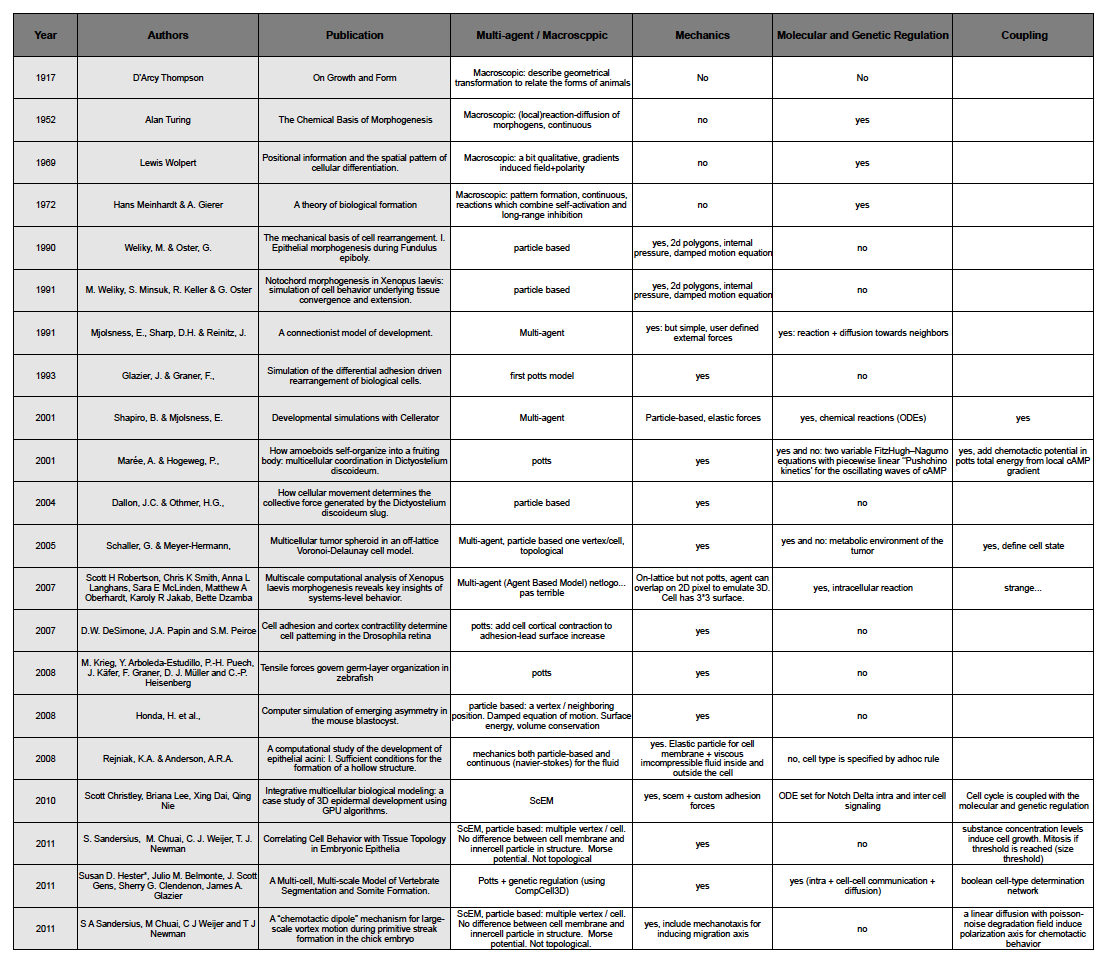
\includegraphics[width=0.95\textwidth]{../../images/Development_Review/theoretical_model/review3_part1.png}
\end{center}
\caption{\textbf{Summary table of the developmental models and principles reviewed in Section 2.} (Part I)}
\label{theoretical_model_review1}
\end{figure}
\begin{figure}
\begin{center}
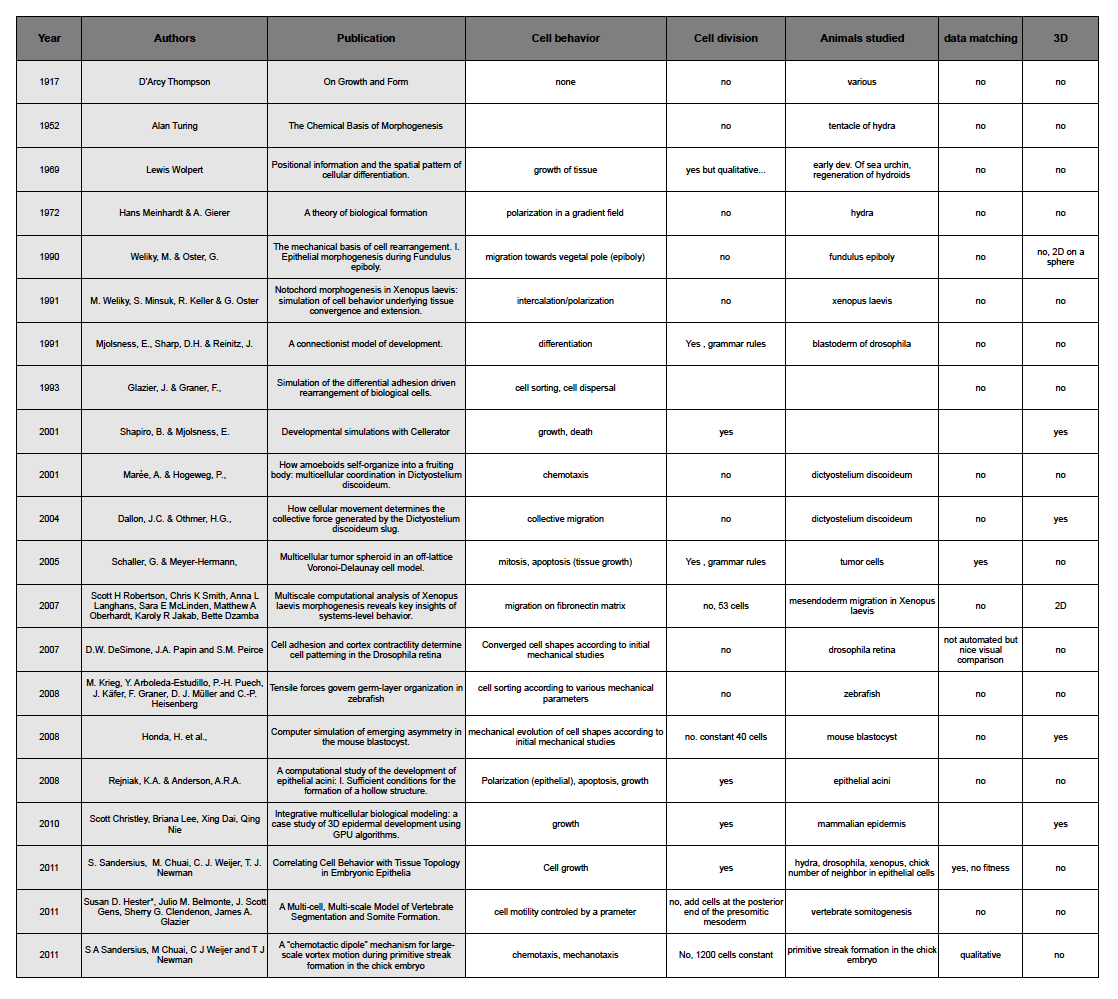
\includegraphics[width=0.95\textwidth]{../../images/Development_Review/theoretical_model/review3_part2.png}
\end{center}
\caption{\textbf{Summary table of the developmental models and principles reviewed in Section 2.} (Part II)}
\label{theoretical_model_review2}
\end{figure}

\subsection{Overview of the MECAGEN Modeling Principles }

  In the next three chapters, we explain the model that we have designed to contribute to the objective of the MECAGEN project.  
\begin{itemize}
	\item Chapter 3 describes how we express and calculate the mechanical interactions and behavioral properties of the cells. It presents a discrete-element model using one particle per cell driven by an overdamped equation of motion that can be summarily written $\lambda \vec{v_i} = \vec{F_i^P}+\vec{F_i^A}$, where $\vec{v_i}$ is the velocity of one cell $i$, $\vec{F_i^P}$ represents "passive" interaction forces controlling cell stiffness and adhesion, and $\vec{F_i^A}$ represents "active" interaction forces, based on polarization axes, which create protrusive activity or apical constriction. These forces are calculated by summing over a neighborhood $\mathcal{N}_i$ containing nearby cells that are in contact with cell $i$. This neighborhood is itself defined by a metric and topological criteria. $\vec{F_i^P}$ is a \textit{relaxation} force derived from an attractive/repulsive, elastic-like interaction potential. $\vec{F_i^A}$ is a \textit{behavioral} force moving the swarm configuration away from equilibrium.
	\item Chapter 4 deals with chemical signaling and gene regulatory networks. The goal is to briefly explain the principles of gene regulatory networks (GRNs), describe the components of GRN models, and give examples. In the present work, our particular objective was to design a simple and easily computable model of the molecular and genetic interactions that occur during development. Our model is articulated around three types of rules: rules driving the dynamics of intracellular gene/protein reactions, rules driving the dynamics of cellular secretion and transduction and rules driving the dynamics of extracellular reactions, transport and diffusion. They are expressed in a chemical kinetic framework by ODEs of the type $dp/dt=f(p,g,q,r)$, where $p$ represents protein concentrations, $g$ gene expression level, $q$ external ligands, and $r$ membrane receptors. Extracellular reactions, transport and diffusion of ligands are also taken into account via PDEs involving $\partial q/\partial t$ and fluxes $\vec{J}=-D\vec{\nabla}q$.
	\item Finally, the first steps toward building a complete morphogenetic platform integrating mechanics and genetics will be laid out in Chapter 5. A simplified "cell behavior ontology" (CBO) is proposed. It relates on the one hand \textit{cell states}, determined by the concentrations of certain proteins, and on the other hand \textit{cell behaviors}, determined by biomechanical parameters.
\end{itemize}
\begin{figure}
\begin{center}
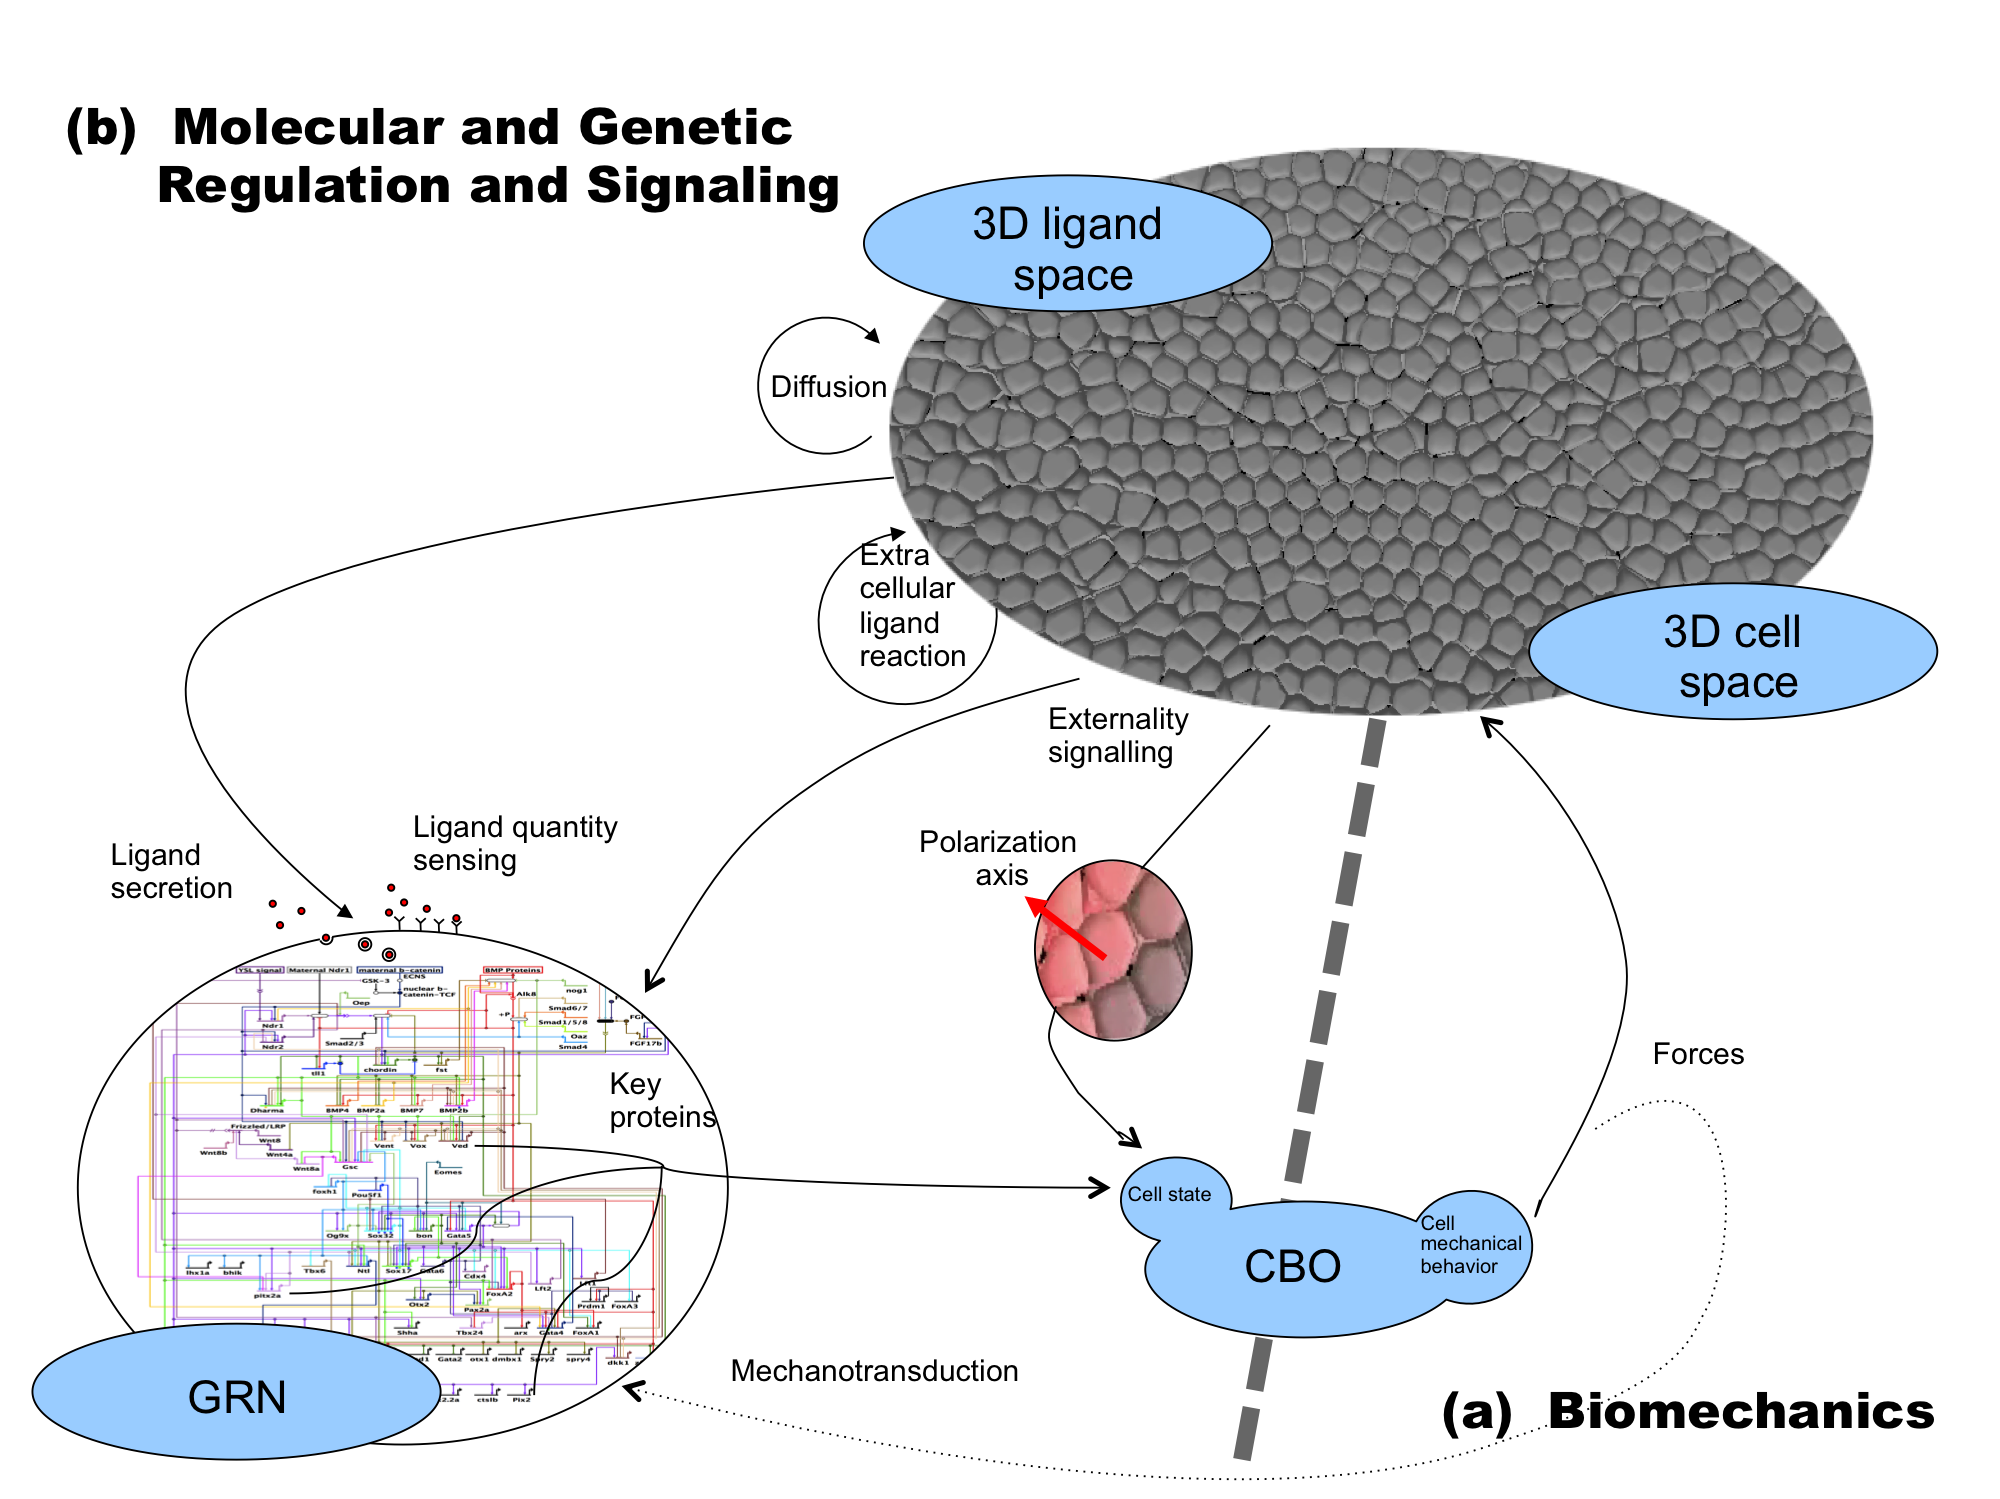
\includegraphics[width=0.95\textwidth]{../../images/MECAGEN/schematic/schemaMECAGEN.png}
\end{center}
\caption{\textbf{General diagram of the MECAGEN project.} a: Biomechanical processes, including a "passive" and "active" forces (see summary of Chapter 3 above). b: Molecular/genetic regulation and signaling processes, including gene regulation networks, intracellular protein concentrations, extracellular ligands secretion, diffusion and binding.}
\label{schematic_mecagen}
\end{figure}
